\chapter{Misc}
\label{sec:misc}
% Old Ch. 10

\textit{Of less importance}
\vspace{6mm}

\section{Fonts}

\section{Web Hosting}

\section{Optional QOL tools for MacOS}
\label{sec:iterm}
\textit{Of less importance, covered in \href{https://www.youtube.com/watch?v=ZIBEVGrtiVA&list=PLjGmdnqrOKuYXiu7lgG5HW71jPEUd1XCm&index=7}{video 6a of the series}}
\vspace{6mm}

Refer to \href{https://www.youtube.com/watch?v=ZIBEVGrtiVA&list=PLjGmdnqrOKuYXiu7lgG5HW71jPEUd1XCm&index=7}{the video}\footnote{Link: \url{https://www.youtube.com/watch?v=ZIBEVGrtiVA&list=PLjGmdnqrOKuYXiu7lgG5HW71jPEUd1XCm&index=7}}.

Here is an outline on what is installed.
\begin{itemize}
    \item iTerm2 - \url{https://iterm2.com/}
    \item oh my zsh - \url{https://ohmyz.sh/}
    \item Colour theme - \url{https://github.com/MartinSeeler/iterm2-material-design}, follow the documentation in the README and apply the colour theme to your terminal
    \item Changing the theme of oh my zsh by editing the \texttt{.zshrc} file by running \texttt{open .zshrc}. Edit one of the lines to \texttt{ZSH\textunderscore THEME = "ys"} 
    \item tldr pages - \url{https://tldr.sh/}

\end{itemize}

\section{Optional VS Code Plugins}
\textit{Of less importance}
\vspace{6mm}

Refer to the very last section of \href{https://github.com/OscarMui/setup-cheetsheet-macos}{my setup cheetsheet}\footnote{Link: \url{https://github.com/OscarMui/setup-cheetsheet-macos}} (last part works for all operating systems) Not all of them are useful to you, just choose ones that you like.

Here is an outline on something that might be useful. These are the extension IDs, copy and paste them in the search extensions box to find them.

\begin{itemize}
    \item sdras.night-owl (A cooler theme)
    \item aaron-bond.better-comments (Coloring comments with //!, //TODO, //?)
    \item bierner.markdown-preview-github-styles (Preview of .md files) 
    \item adpyke.codesnap (Beautiful screenshots, suggest checking codesnap.transparentBackground)
    \item mhutchie.git-graph (View Git history by Git Graph: view Git Graph (git log))
\end{itemize}

\section{Why?}
\label{sec:rationale}

I would like to explain what I would like to achieve this piece of notes in this section, so as to manage your expectations.
\vspace{6mm}

\textbf{TL;DR: I believe what you will learn is useful in some way if you would like to pursue jobs related to IT, or dig deeper in programming and Computer Science. Knowledge in Git is also crucial for Maths, Statistics and science subjects undergraduates as they also need to write code sometimes as a group.}

\subsection*{Why making websites?}

Websites are cross-platform, meaning that they can be opened on different kinds of devices, basically any device with a browser. From mobile phones to laptops and desktops, no matter which operating system they are on (e.g. Windows, MacOS, Linux, Android, iOS).

On the other hand, you can only code mobile apps for one specific platform\footnote{Flutter or React Native are exceptions, but they have their downsides}. For instance, Android apps I built cannot be installed on iOS devices unfortunately.

\subsection*{Command line and Git}

Learning how to make a website is actually just a facade. The most important thing that I think you will take away with is the knowledge on command line and Git.

Knowing how to use the command line is important because you can work more efficiently if you are proficient at command line tools. And you will come across some situations where only command line is available (e.g. when accessing a remote server). 

Git is important because it allows you to work and communicate with people using just a few simple commands. By following its rules and conventions, you can work with others efficiently, without having to send zip files back and forth through emails. 

\subsection*{Can I use GitHub Desktop or similar visualisation tools in place for command line?}
\label{sec:githubdesktop}
Not really. Git is a command line tool and is best used through the command line. Again, you will come across some situations where only command line is available (e.g. when accessing a remote server). 

However, it is acceptable if you just want to visualise the git commit history. Just don't run any commands using those visualisation software. (See \cref{sec:sublime})

\subsection*{Why not plain HTML?}

Pug.js allows the use of templates, hence there is no need to modify every page file whenever we need to something that every page has in common. Pug.js also allows the use of variables, so that we can control what to be rendered based on the situation, hence providing a basis for building dynamic websites. (see \cref{sec:limitations} Scope and limitations)

Moreover, using my template allows you to learn about the conventions of Node.js frameworks, such as how \texttt{npm install} works, and the use of files such as \texttt{package.json}. Knowing these makes it slightly easier for you to learn state-of-the-art Node.js frameworks (e.g. React, Angular, Discord.js).

\subsection*{Responsiveness}

Mobile devices are common nowadays, so our website has to cater for screens with different sizes, from those as small as mobile phones to those as big as projectors. 

A website is responsive if it can rearrange its elements for easy readability based on the screen size and orientation. The use of Bootstrap makes our website responsive.
\vspace{6mm}

I think the following summarises what we talked about in this section. I think building websites is half of the course while another half is about command line and Git.

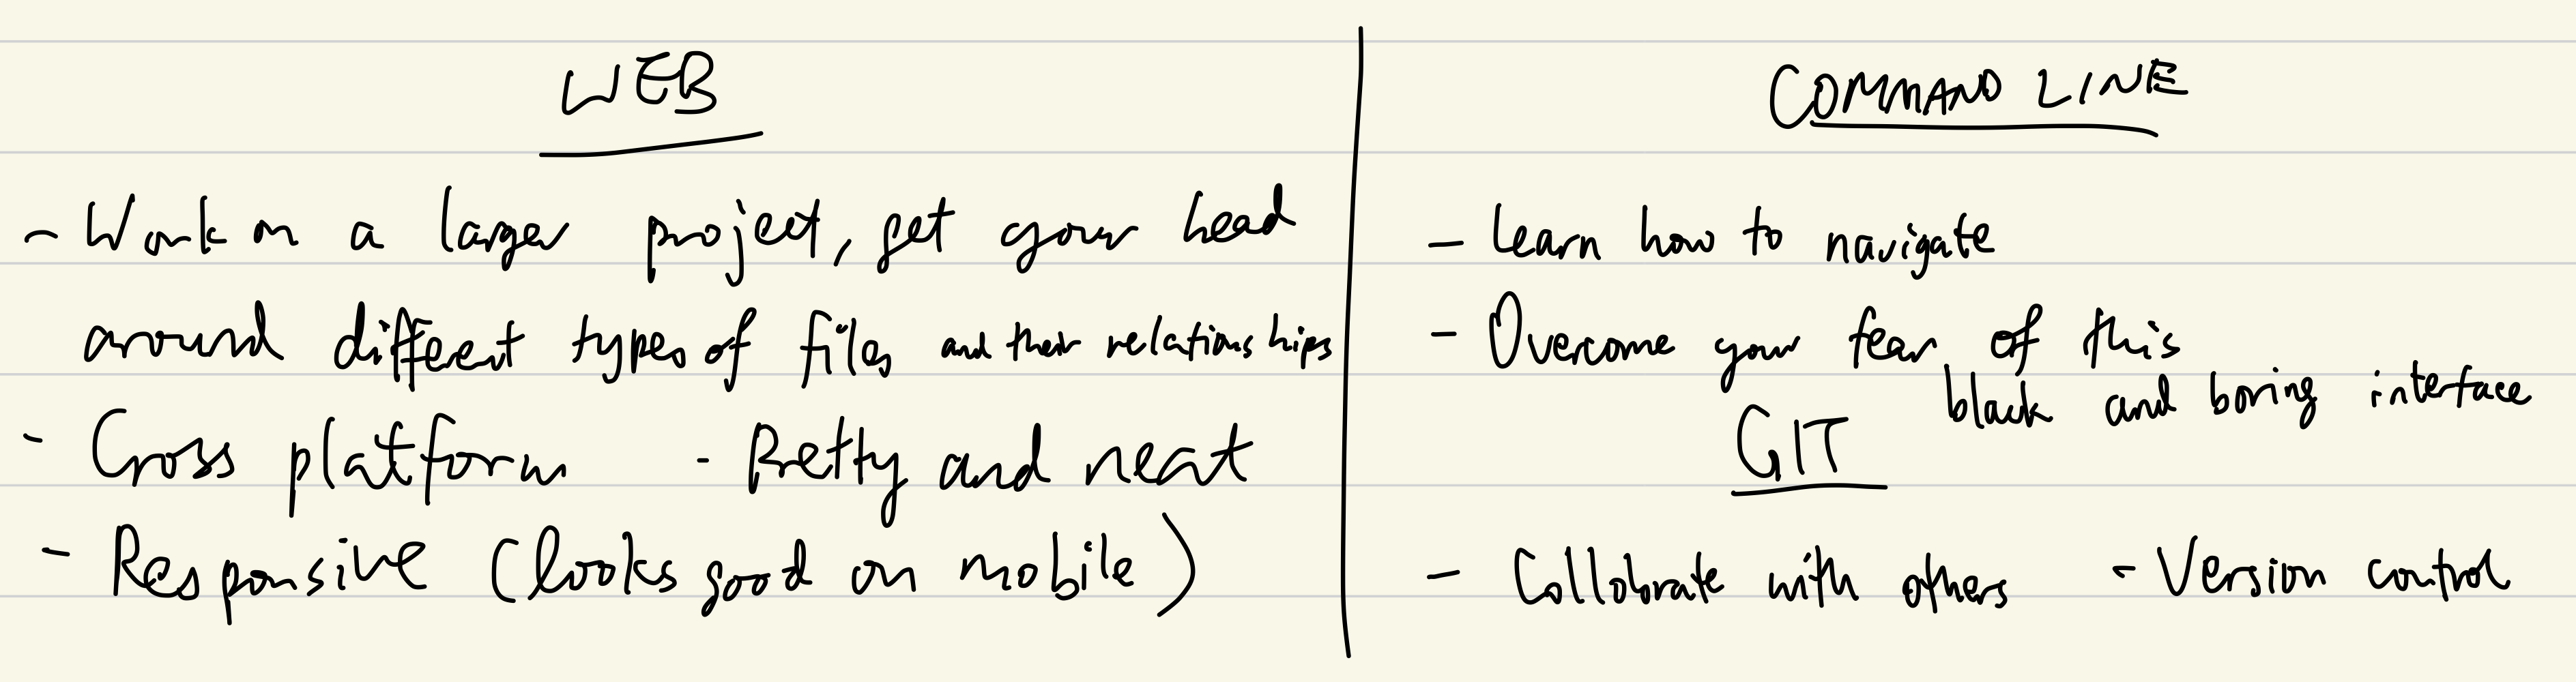
\includegraphics[width=15cm]{images/ch0-summary-of-course.png}

\section{Scope and limitations}
\label{sec:limitations}
We will focus on styling and making the web page responsive. Our styles would be neat, but without too many animations, making them suitable for serious applications such as e-commerce, or a self-introduction website, while not too suitable for websites for fun.

We will not focus much on providing interactions with users, so JavaScript is not used throughout this piece of notes, however, you could definitely add interactions on your own.

The websites that we are making are static. That means we cannot interact with back-end servers and databases securely, while dynamic websites can. A framework that you can learn after mastering this piece of notes is \href{https://expressjs.com/}{ExpressJS}.\footnote{Link: \url{https://expressjs.com/}}